\documentclass[10pt]{article}

% --- BASIC PACKAGES ---
\usepackage[utf8]{inputenc}
\usepackage{amsmath, amssymb, amsfonts} % For advanced math
\usepackage{graphicx}                   % For including images
\usepackage[a4paper, margin=1in]{geometry} % Set page margins
\usepackage{hyperref}                   % For clickable links and citations
\hypersetup{
    colorlinks=true,
    linkcolor=blue,
    filecolor=magenta,      
    urlcolor=cyan,
    citecolor=red,
}

% --- CHINESE LANGUAGE SUPPORT ---
\usepackage{ctex} % Kept from your original for Chinese characters

% --- BIBLIOGRAPHY (using biblatex) ---
% Switched to biblatex for modern citation management. It works well with \citet.
% You will need to compile with: pdflatex -> biber -> pdflatex -> pdflatex
\usepackage[backend=biber,style=gb7714-2015ay]{biblatex}
%biblatex宏包的参考文献数据源加载方式
\DefineBibliographyStrings{english}{
  andincite = {和},
  andincitecn = {和},
  andothersincite = {等},%adddot才能避开标点追踪
  andothersincitecn = {等}, }
\addbibresource{ref.bib} % Assumes your bibliography file is ref.bib

% --- CUSTOM COMMANDS ---
\newcommand{\his}{\textsuperscript{\ddag}}

% --- DOCUMENT METADATA ---
\title{Turbulence phenomenology \\ \large The Gioia\his way.}
\author{刘宁 \\ \textit{浙江大学}} % Institute is often placed under the author
\date{\today}


\begin{document}

\maketitle

\begin{abstract}
This document outlines the phenomenology of turbulence following the approach developed by Gioia and coworkers. We review the formulation for the velocity scale, the local shear stress model, and its unification across different flow regions, drawing comparisons to other established models.
\end{abstract}


\section{Velocity Component at the $s$ Scale}

The squared velocity component at a scale $s$ can be expressed through an integral of the energy spectrum, either over the spatial scale $\sigma$ or the wavenumber $k$:
\begin{align*}
    u_s^2 = \int_0^s E(\sigma) \sigma^{-2} d\sigma = \int_{1 / s}^{\infty} E(k) dk
.\end{align*}
The energy spectrum $E$ is modulated by correction functions for the dissipative range ($\mathbf{c_d}$) and the energy-containing range ($\mathbf{c_e}$): \footnote{Note: \citet{gioiaFriction2006} use the form $\mathbf{c_e} \left( \sigma / R \right) $. We notice that $R / \sigma = Rk$, so to maintain a uniform style for $\mathbf{c_e} $, we define it as $\mathbf{c_e} \left( R / \sigma \right) $.}
\begin{align*}
    E(\sigma) &\sim \varepsilon^{2 / 3} \sigma^{5 / 3} \mathbf{c_d} \left( \frac{\eta}{\sigma} \right) \mathbf{c_e} \left( \frac{R}{\sigma} \right) \\
    E(k) &\sim \varepsilon^{2 / 3} k^{-5 / 3} \mathbf{c_d} (\eta k) \mathbf{c_e} \left( \frac{1}{Rk} \right).
\end{align*}
The correction functions are given as:
\begin{align*}
    \begin{cases}
        \mathbf{c_d}\left( x \right)  = \exp\left( -\beta_d x \right) \\
        \mathbf{c_e} \left( x \right) = \left( 1+\beta_e x^{-2} \right) ^{-17 / 6} 
    \end{cases}
.\end{align*}
The form of $\mathbf{c_d}$ is from \citet{gioiaFriction2006}, while $\mathbf{c_e}$ is taken from von Kármán. In the inertial range, where $\eta \ll s \ll R$, both correction terms approach $1$.\footnote{Why does adjusting the coefficients for the dissipative and energy-containing ranges fail to derive the common $-1$ scaling law? See \cite{nikora1999prl} 假设当涡体尺度由外区标度控制$1 / H \ll k \ll 1 / z$时,引入$\varepsilon(k) \sim u_{\tau }^3 k$.}

\section{The Uniform Form of Velocity $u_s$}

Let $\xi = sk = s / \sigma$. We can rewrite $u_s$ in a uniform representation:
\begin{align*}
    u_s \sim \left( \varepsilon s \right) ^{1 / 3} \left[ \int_1^{\infty} \xi^{-5 / 3} \mathbf{c_d}\left( \frac{\eta}{s} \xi \right) \mathbf{c_e} \left( \frac{R}{s} \xi \right) d\xi \right]^{1 / 2}  \triangleq \left( \varepsilon s \right) ^{1 / 3} \sqrt{\mathcal{I} } 
.\end{align*}

\paragraph{Takeaway Message.}
\begin{itemize}
    \item In the inertial range ($\eta \ll s \ll R$), the velocity scales as $u_s \sim \left( \varepsilon s \right) ^{1 / 3} $.
    \item The problem of determining the characteristic velocity $u_s$ of an eddy of size $s$ is transformed into an analysis of the correction function $\mathcal{I}\left( \eta / s, R / s \right)$, defined as:
    \[
        \mathcal{I}\left( \frac{\eta}{s}, \frac{R}{s} \right)  \triangleq \int_1^{\infty} \xi^{-5 / 3} \mathbf{c_d}\left( \frac{\eta}{s} \xi \right) \mathbf{c_e} \left( \frac{R}{s} \xi \right) d\xi.
    \]
\end{itemize}

\section{The Phenomenology Big Picture}

The model is built upon the concept of an energy cascade.
\begin{itemize}
    \item \textbf{Energy Cascade}: The rate of energy transfer is constant across scales.
        \begin{align*}
            u_s^3 / s \sim u_R^3 / R
        .\end{align*}
        \begin{itemize}
            \item With $\varepsilon \sim u_R^3 / R$, the Kolmogorov scale is $\eta = \left( \nu^3 / \varepsilon \right)^{1 / 4}\sim R\cdot Re^{-\frac{3}{4}} $. 
            \item With $\varepsilon  \sim {u_{\tau }^3}/{\kappa y}$ and $u_s\sim \left( \varepsilon s \right) ^{1 / 3} $, for inertial range eddies (especially in the log layer, where $s \sim y$)\footnote{Therefore, in the outer layer, ignoring the viscous sublayer, the eddies that mix momentum naturally have a characteristic velocity of $u_{\tau }$.}:
                $$u_s \sim u_{\tau } \left( s / y \right) ^{1 / 3} \sim u_{\tau}.$$ 
            \item \textbf{Inconsistency in $C_f$ scaling (?)}: \citet{gioiaFriction2006} express the friction factor as $C_f \sim u_s / V \sim u_{\tau } / V$. However, considering the definitions of friction velocity and friction factor, we get $C_f \sim \tau / V^2 \sim u_{\tau }^2 / V^2$.
        \end{itemize}
\end{itemize}


\section{The Gioia Way: Local Shear Stress Model}

Eddies of size $(u_s, s)$ that straddle a wetted surface $W_y$ generate a shear stress $\tau$. The model conceptualizes this as the product of the rate of momentum transfer ($v_n$) and the magnitude of the momentum being transferred ($v_t$).
\begin{itemize}
    \item $v_n$ represents the rate at which an eddy transfers momentum, which depends on its characteristic velocity ($\sim u_s$).
    \item $v_t$ represents the amount of momentum the eddy can transfer, which depends on the momentum difference across the wetted area ($\propto \frac{\partial u}{\partial y}\cdot s $).
\end{itemize}
The shear stress is modeled as:
\begin{align*}
    \tau \sim \rho v_t v_n
.\end{align*}

\begin{figure}[ht!]
    \centering
    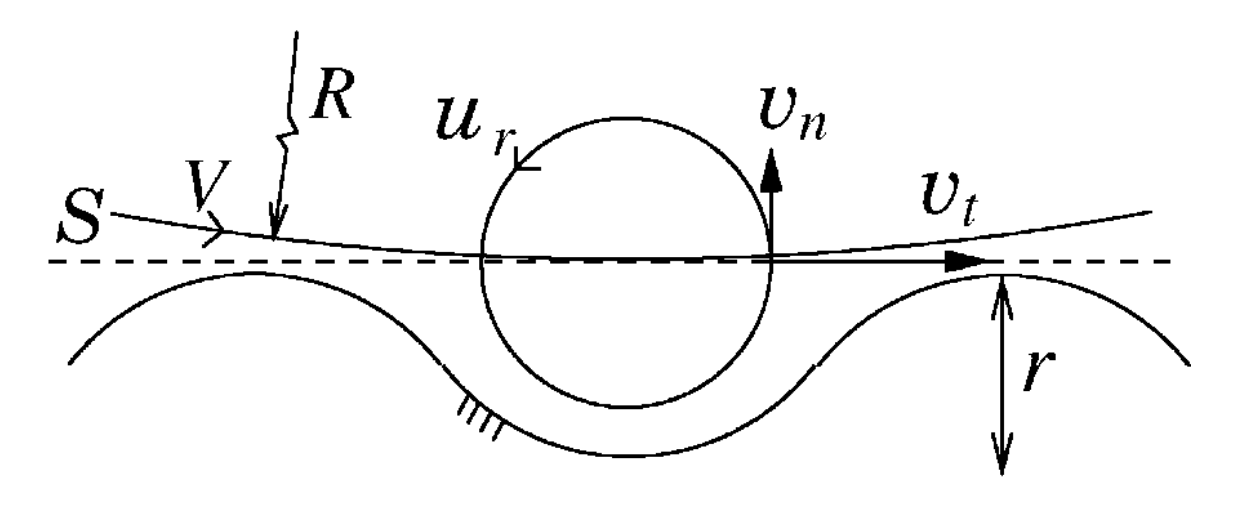
\includegraphics[width=0.4\textwidth]{./figures/eddies.png}
    % \caption{Schematic of eddy phenomenology \cite{gioiaprl2001}.}
    \label{fig:-figures-eddies-png}
\end{figure}

The model is applied differently depending on the location:
\begin{itemize}
    \item \textbf{Local wall shear stress model} \cite{gioiaFriction2006}: $v_t \sim V$, $v_n\sim u_{k_s+a\eta}$.
    \item \textbf{Local water column shear stress model} \cite{gioiaMVP2010}: $v_t\sim u(y+s) - u(y-s)\approx 2s u'(y) \sim 2y\cdot u'(y)$, $v_n \sim u_y$.
\end{itemize}

\begin{figure}[!htb]
    \centering
    \begin{minipage}{.5\textwidth}
        \centering
        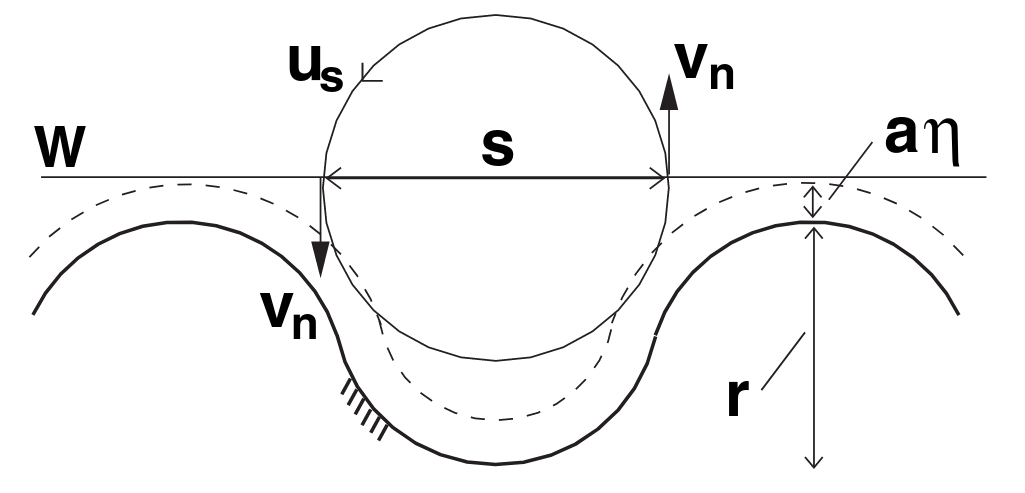
\includegraphics[width=0.7\textwidth]{./figures/wall-shear.png}
        \caption{Wall shear stress model.}
        \label{fig:wall-shear}
    \end{minipage}%
    \begin{minipage}{0.5\textwidth}
        \centering
        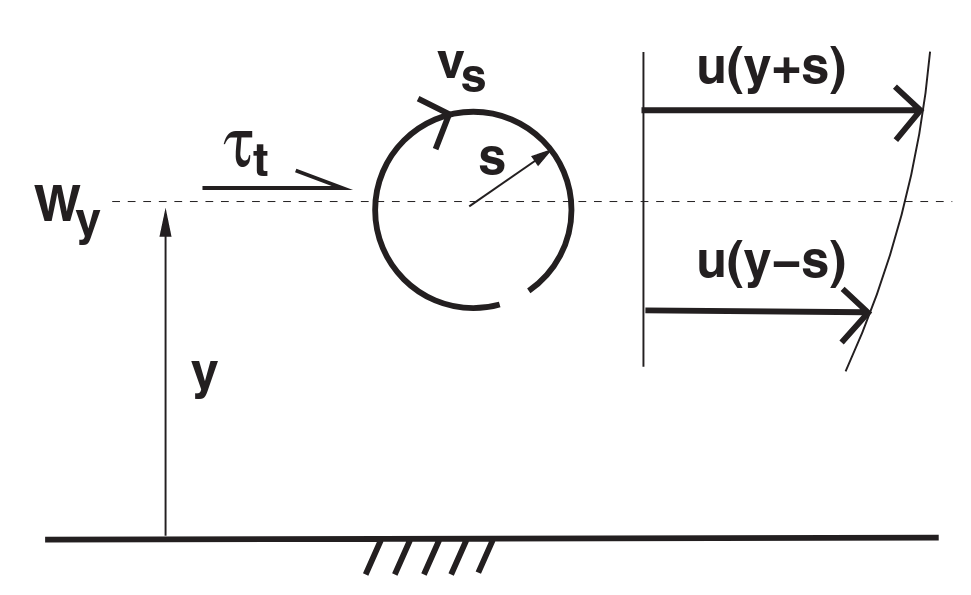
\includegraphics[width=0.7\textwidth]{./figures/column-shear.png}
        \caption{Water column shear stress model.}
        \label{fig:column-shear}
    \end{minipage}
\end{figure}


\section{Unifying the Local Shear Stress Model}

\subsection{A Unified Picture}

\begin{figure}[htpb]
    \centering
    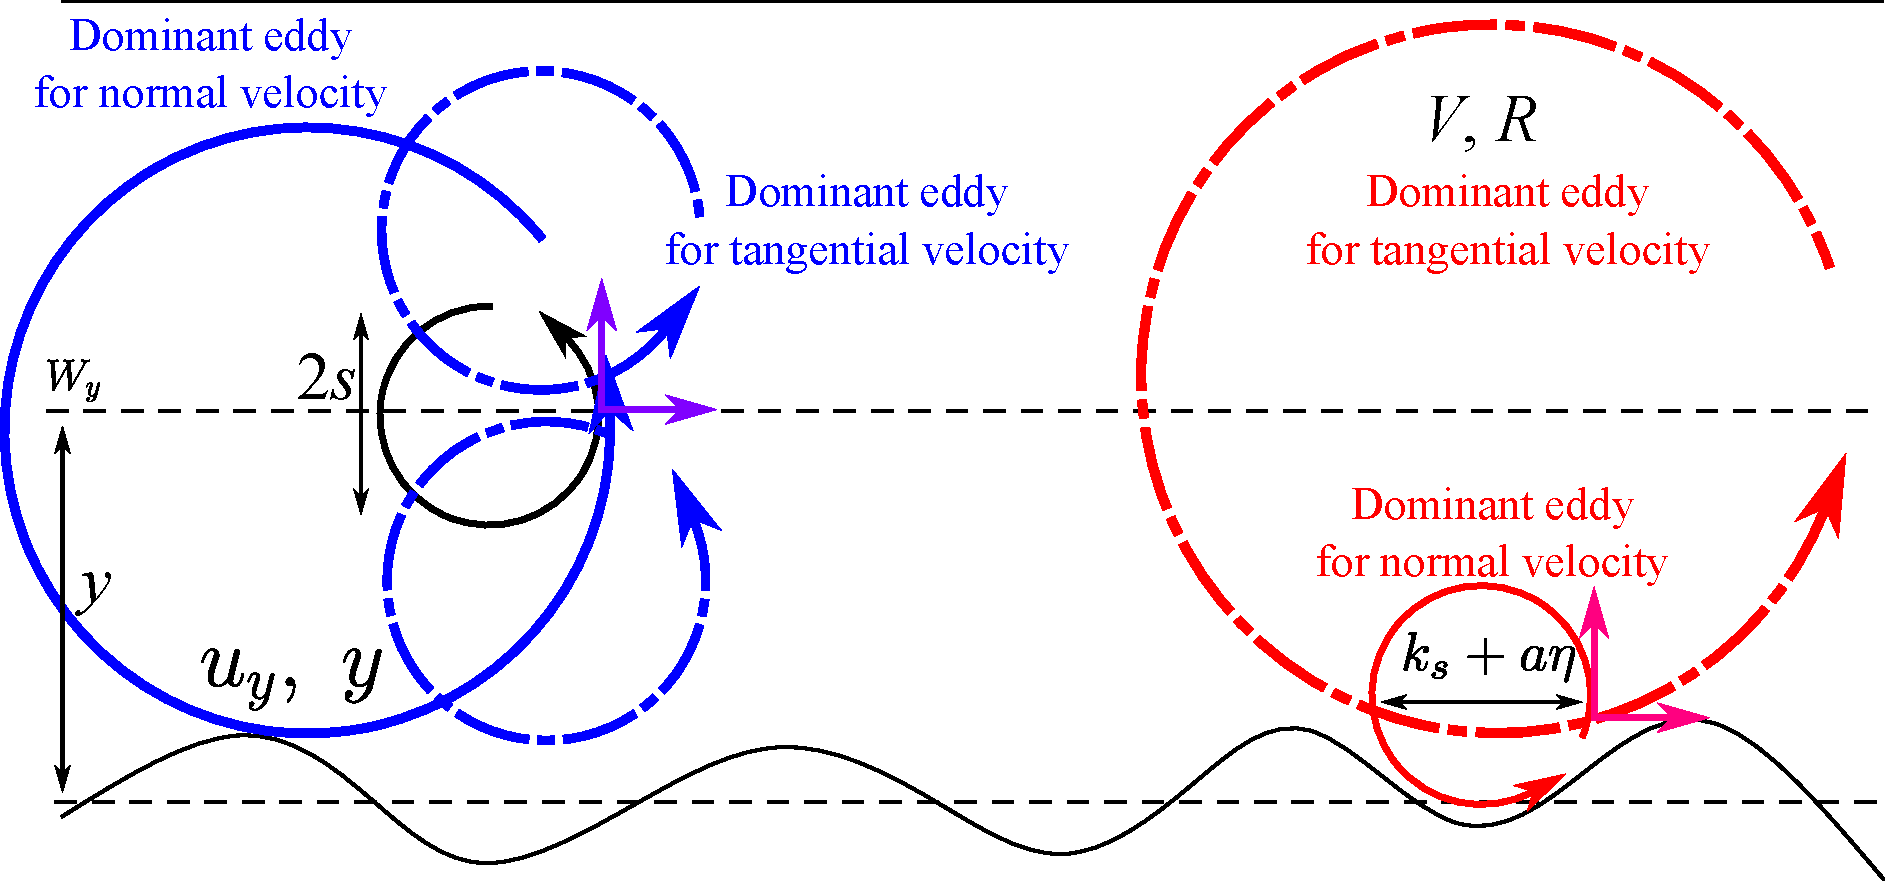
\includegraphics[width=0.8\textwidth]{./figures/unify-gioia-model.pdf}
    \caption{The unified picture of the Gioia model.}
    \label{fig:-figures-unify-gioia-model-pdf}
\end{figure}

The core idea is to define the momentum "transporter" ($v_n$) and the "cargo" ($v_t$) based on the eddy's location and scale.
\begin{itemize}
    \item \textbf{The Transporter ($v_n$)}: Near the bed, the characteristic eddy size is controlled by both the roughness height $k_s$ and the viscous sublayer thickness $a\eta$, so $s = k_s + a\eta$\ddag. In the outer region, the characteristic eddy size is governed by the distance from the wall, $s\sim y$.\footnote{Townsend's attached-eddy hypothesis posits a similar series of self-similar eddies whose characteristic scale is proportional to the wall distance. This might be viewed as a special case considering only outer-layer eddies, which is why the attached-eddy model is primarily applicable to the log-law region \cite{aemmarusic2019}.}
    
    \item \textbf{The Cargo ($v_t$)\his}: The eddies responsible for the $v_n$ component act as momentum transporters. Their spatial scale determines the amount of momentum, $v_t$, they can carry.\footnote{Because for a given eddy spatial scale $s$, the velocity gradient covered over this distance is a function of $s$.}
        \begin{itemize}
            \item Once the eddy scale $s$ is determined, are $v_n$ and $v_t$ determined simultaneously? If so, a model of large eddies superimposed on small eddies may no longer be necessary. We would only need to introduce the "transporter" eddies, similar to the attached-eddy model.
            \item The momentum difference that can be transported due to the velocity gradient in the outer region is:
            $$v_t \sim 2s u'(y) \sim 2y \cdot u'(y).$$
            \item The momentum difference near the wall\his is\footnote{This leads to a Strickler-type relation for transitional roughness: $\tau_0 \propto \left( k_s / R \right) ^{\frac{1}{3}} \rho V^2 $.}:
            $$\lim_{y \to 0} v_t \sim \left( k_s + a\eta \right) \lim_{y \to 0} u'(y) =  \frac{(k_s + a \eta)u_{\tau}^2}{\nu} \sim (k_s + a\eta) \frac{\left( k_s / R \right)^{\frac{1}{3}} V^2}{\nu}.$$
            上述式子显然不单单scale with 平均流速$V$,而是与$Re = \left( k_s + a\eta \right) V / \nu$ 相关。因此在考虑内标度范围的近壁面区域,涡体能够交换的动量差无法直接以\citet{gioiaprl2001}中大小涡体叠加的模型中的 $V$ 作为特征速度\footnote{这是附着涡模型带过来的陷阱,未考虑到黏性效应依赖雷诺数。“In fact, Ref. \citep{Hwang2016} showed that there is nontrivial Reynolds-number dependent viscous effect on the spectra of the footprint of self-similar energy-containing motions (i.e., the near-wall part of the motions).”}。
        \end{itemize}
\end{itemize}


\subsection{Eddies as Momentum Diffusion Systems}
An eddy of scale $(V, R)$ can be viewed as a momentum diffusion system $\mathcal{D}_e \propto VR$ \cite{ocfjfm2024}.\footnote{At this point, we have moved beyond the visualization of fluid flow and are no longer trying to capture abstract eddies from the flow field. This perspective is similar to Prandtl's mixing length theory.} This perspective highlights a fundamental contrast:
\begin{itemize}
    \item Laminar flux is driven by molecular diffusion ($\propto \nu$).
    \item Turbulent flow is driven by diffusion by the largest eddies and recirculation cells ($\propto VR$).
    \item The Reynolds number, $Re = \frac{VR}{\nu}$, represents the ratio of these turbulent to laminar driving mechanisms.
\end{itemize}
The momentum flux $F$ generated by an eddy $(V, R)$ is given by\footnote{The derivation for the second case in the paper might risk being a circular argument.} \cite{ocfjfm2024}:
\begin{align*}
    F \sim \rho \left[ (VR)^2 \right] '\sim -\rho \int_0^{R}  \mathcal{D}_e \frac{\partial u}{\partial y} dz
.\end{align*}

\begin{figure}[ht!]
    \centering
    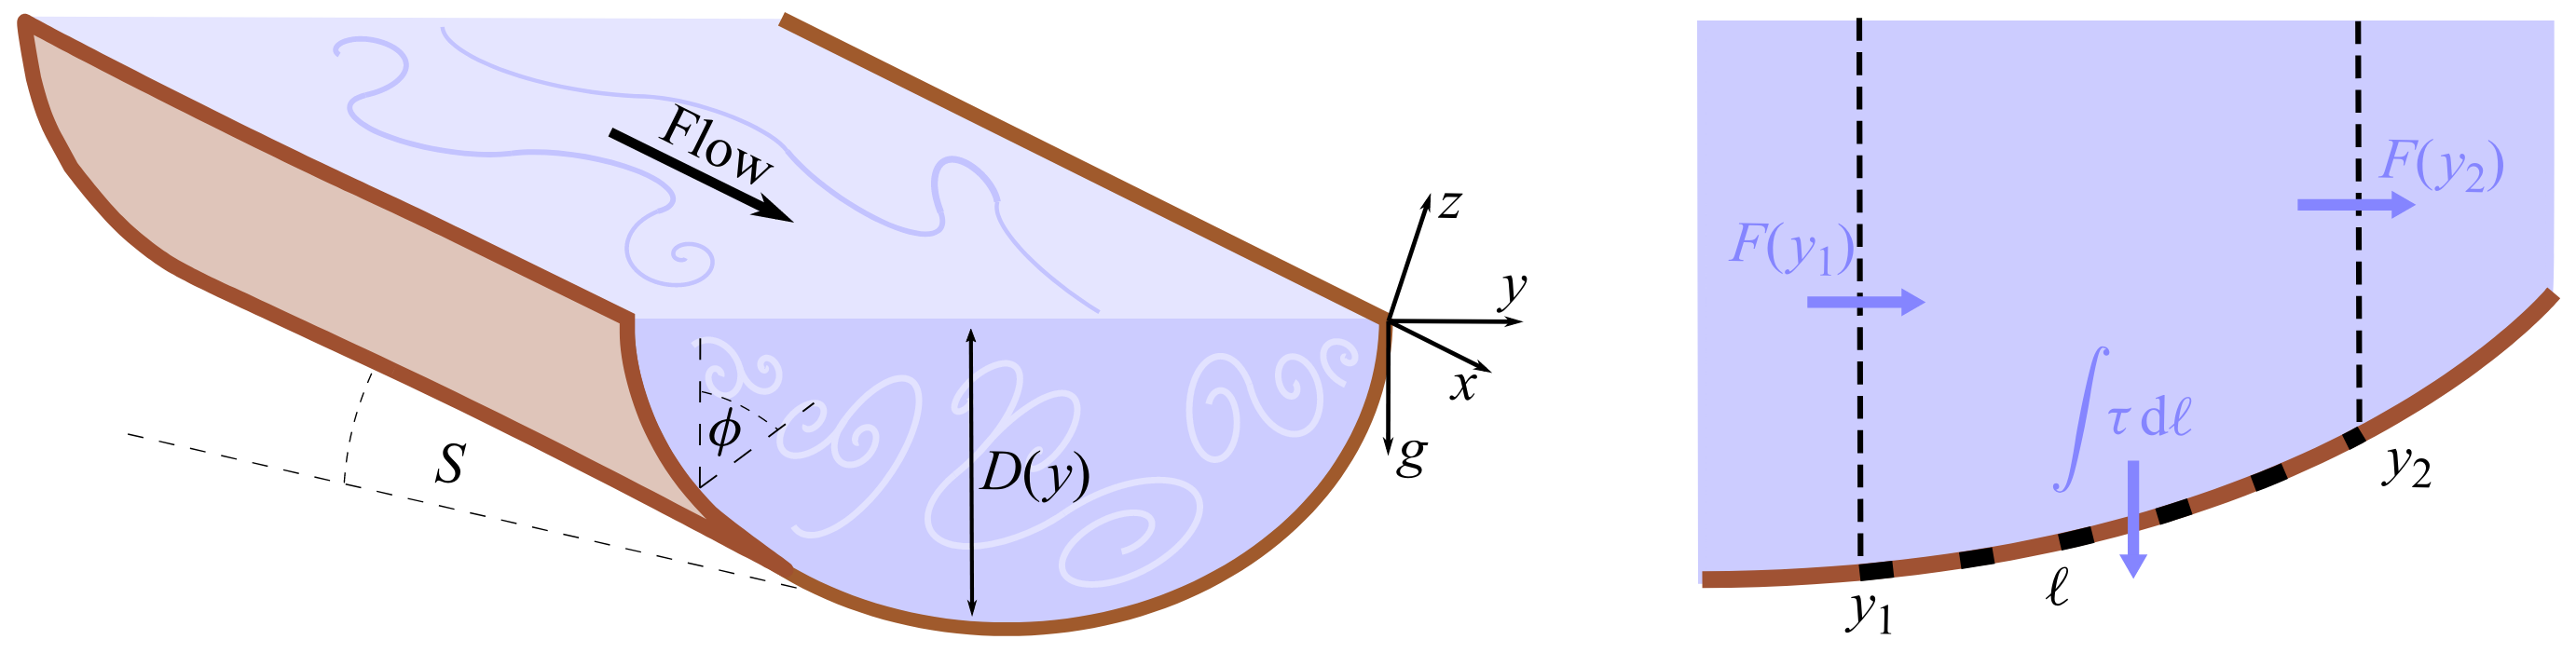
\includegraphics[width=0.6\textwidth]{./figures/momentum-flux.png}
    \caption{Momentum balance in a portion of the channel, from \cite{ocfjfm2024}.}
    \label{fig:-figures-momentum-flux-png}
\end{figure}

\section{The Gioia Eddy Model vs. Attached Eddy Model}
\textit{(Content to be added.)}

\section{The Gioia Eddy Model vs. Eddy Viscosity Model}
\textit{(Content to be added.)}

\section{The Gioia Eddy Model in the Perspective of the Time-Averaged Field}
\textit{(Content to be added.)}

\section{The Gioia Eddy Model vs. LSM/VLSM}
\subsection{The ``-1'' scaling law in perspective of turbulence phenomenology}
\citet{nikora1999prl} 借助涡体能量串级的唯象学解释:特定尺度$\frac{1}{k}$ 的涡体能量通量等于所有更大尺度涡体能量通量和自身动量通量的叠加,直至到达惯性区尺度的涡体(外标度不再起作用,局部各向同性,OK41理论)动量通量为常值$\varepsilon_d$。

\begin{figure}[htpb]
    \centering
    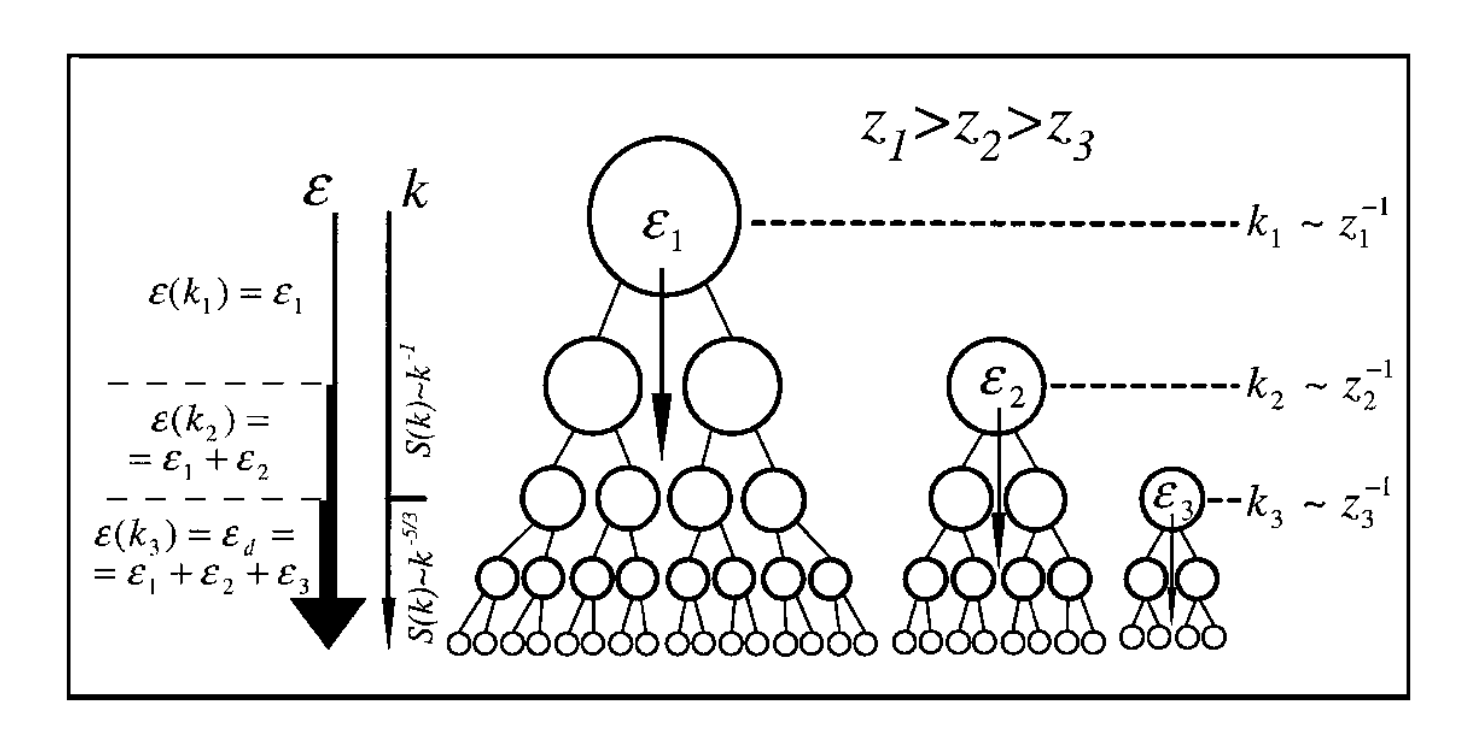
\includegraphics[width=0.8\textwidth]{./figures/energy-cascade.png}
    \caption{The effect of superposition of energy cascades measured at $z_3$ and initiated at all possible $z$. \cite{nikora1999prl}}
    \label{fig:-figures-energy-cascade-png}
\end{figure}

将外标度区域的涡体能量通量$\varepsilon(k)$

\begin{figure}[htpb]
    \centering
    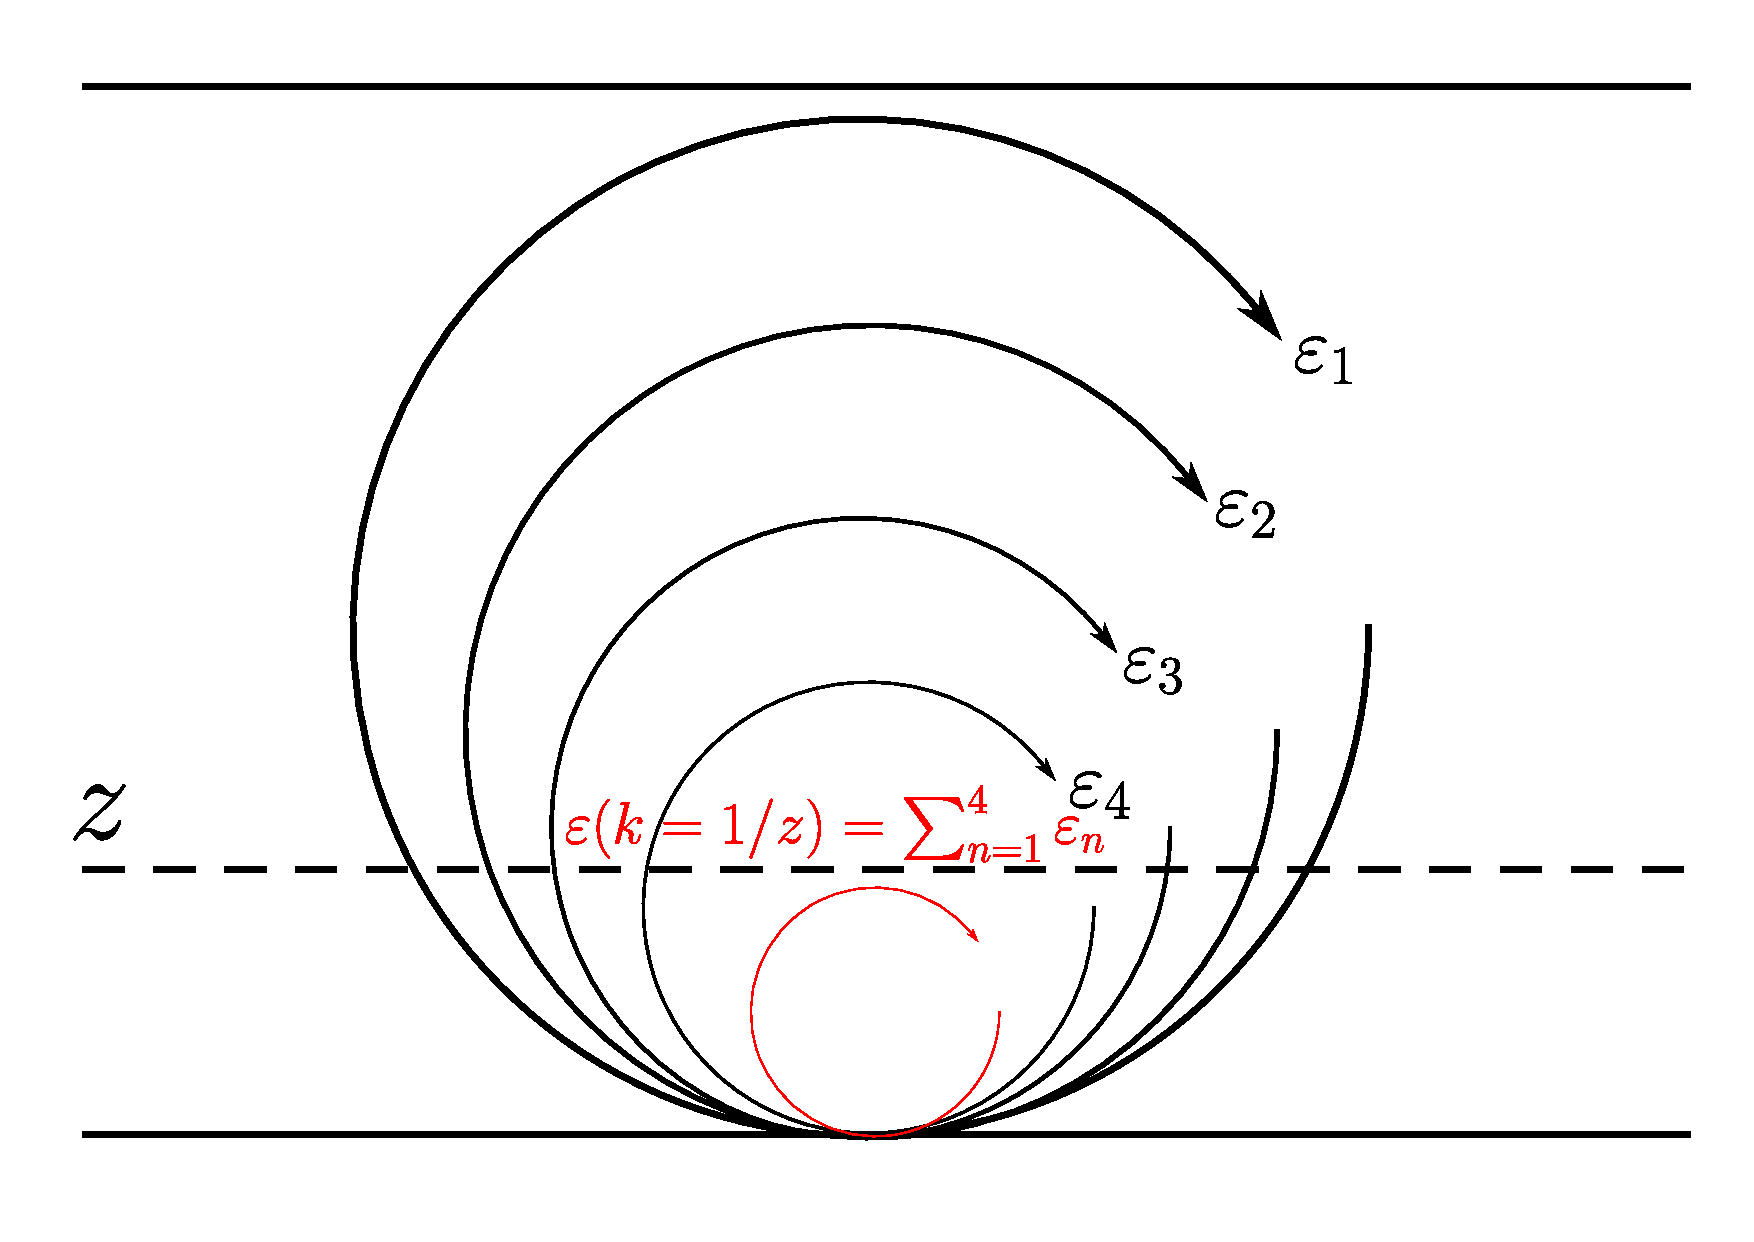
\includegraphics[width=0.6\textwidth]{./figures/cascade.pdf}
    \caption{Outer region energy flux cascade.}
    \label{fig:-figures-cascade-pdf}
\end{figure}
\section{Future Vision}
\begin{itemize}
    \item The local shear stress model $\implies$ a new sub-grid stress model.
    \item A new sub-grid stress model $\implies$ a mesh optimizer.
\end{itemize}

% --- BIBLIOGRAPHY ---
\printbibliography[heading=bibintoc, title={References}]

\end{document}
